\documentclass[sigplan,screen]{acmart}

\AtBeginDocument{%
  \providecommand\BibTeX{{Bib\TeX}}}

\setcopyright{acmlicensed}
\copyrightyear{2026}
\acmYear{2026}
\acmDOI{XXXXXXX.XXXXXXX}
\acmConference[CS Capstone '26]{University of Virginia Computer Science Capstone}{May 2026}{Charlottesville, VA}
\acmISBN{978-1-4503-XXXX-X/2026/05}
\settopmatter{printacmref=false}

\usepackage{booktabs}
\usepackage{graphicx}
\usepackage{subcaption}
\usepackage{amsmath}

\title{Graph of Thoughts for Deterministic Graph Reasoning:\\Full Pipeline Study of SFT, Failure Analysis, and Iterative Retraining}

\author{Jonas Lee}
\email{uhz7mq@virginia.edu}
\affiliation{\institution{University of Virginia}\city{Charlottesville}\state{Virginia}\country{USA}}

\author{Neil Morgan}
\email{fwz8ya@virginia.edu}
\affiliation{\institution{University of Virginia}\city{Charlottesville}\state{Virginia}\country{USA}}

\author{Abhinav Pappu}
\email{mzu9pt@virginia.edu}
\affiliation{\institution{University of Virginia}\city{Charlottesville}\state{Virginia}\country{USA}}

\author{Paris Phan}
\email{auj4yx@virginia.edu}
\affiliation{\institution{University of Virginia}\city{Charlottesville}\state{Virginia}\country{USA}}

\author{Andrew Thepvongs}
\email{htf6dp@virginia.edu}
\affiliation{\institution{University of Virginia}\city{Charlottesville}\state{Virginia}\country{USA}}

\renewcommand{\shortauthors}{Lee et al.}

\begin{CCSXML}
<ccs2012>
 <concept>
  <concept_id>10010147.10010178.10010205.10010208</concept_id>
  <concept_desc>Computing methodologies~Natural language processing</concept_desc>
  <concept_significance>300</concept_significance>
 </concept>
 <concept>
  <concept_id>10003752.10003766.10003771</concept_id>
  <concept_desc>Theory of computation~Graph algorithms analysis</concept_desc>
  <concept_significance>300</concept_significance>
 </concept>
</ccs2012>
\end{CCSXML}

\ccsdesc[300]{Computing methodologies~Natural language processing}
\ccsdesc[300]{Theory of computation~Graph algorithms analysis}
\keywords{large language models, graph algorithms, Graph of Thoughts, supervised fine-tuning, DAgger, failure analysis}

\begin{document}

\begin{abstract}
Large language models (LLMs) can imitate algorithmic language but remain brittle on long deterministic graph traces, where early local mistakes compound into global state drift.
This project implements a full Graph of Thoughts (GoT) pipeline that explicitly separates memory from reasoning: a deterministic executor maintains algorithm state while the model predicts one legal next operation at each step.
Beyond a standard SFT baseline, we built benchmark adapters (NLGraph, GLBench), fine-grained failure analysis, and an iterative retraining loop that collects recovery examples from free-running errors and trains a second-stage adapter.
On committed run artifacts, BFS step accuracy improves from 0.00 (base) to 0.62 after SFT.
In iterative pre/post experiments, stage-2 retraining improves BFS from 0.025 to 0.530 step accuracy and DFS from 0.112 to 0.439, with corresponding failure-rate drops of 0.505 and 0.327.
The resulting system is reproducible, modular, and aligned with the original proposal goals of operation-level fidelity, failure localization, and structural extension to larger graph reasoning tasks.
\end{abstract}
\maketitle

\section{Introduction}
Graph reasoning exposes a central weakness in autoregressive language models: sequence modeling can produce fluent algorithm narration without preserving the exact latent state needed for deterministic execution.
In BFS/DFS-style traces, this appears as operation drift, invalid frontier transitions, and hallucinated structural assumptions.
Prior prompting methods such as Chain-of-Thought improve verbalized reasoning, but they do not guarantee state faithfulness under long-horizon constraints~\cite{wei2022cot,liu2023lost}.

Graph of Thoughts (GoT) addresses this by decoupling responsibilities~\cite{got2024,besta2024got}.
The language model is reduced to a local decision policy over legal operation templates, while a deterministic executor tracks and updates global graph state.
In effect, the model acts like an operation selector, not a memory store.
This architecture is well-suited for deterministic graph algorithms where each step can be checked against explicit transition rules.

This final report is intentionally deeper than a standard capstone summary.
It documents not only model metrics but also the engineering decisions reflected in the codebase and iterative debugging history: robust pipeline orchestration, benchmark integration, failure-taxonomy generation, and fault-tolerant DAgger-style retraining.

\textbf{Main contributions.}
\begin{itemize}
  \item A complete data--train--eval stack for BFS/DFS (with Dijkstra support in the executor/training interfaces).
  \item A unified, reproducible pipeline script that runs generation, inference, scoring, failure analysis, and benchmark adapters with run manifests.
  \item An iterative retraining driver that performs pre-eval, error collection, recovery fine-tuning, and post-eval in isolated timestamped directories.
  \item A publication figure suite for baseline vs SFT and BFS/DFS pre/post retraining comparisons, including phase and operation-level failure views.
\end{itemize}

\section{Related Work and Positioning}
\subsection{Prompted reasoning versus state-faithful execution}
Chain-of-Thought prompting improves reasoning articulation but does not enforce executable invariants step-by-step~\cite{wei2022cot}.
For graph algorithms, this distinction is crucial: a model can explain the right idea while still issuing illegal operations.
Our work is positioned closer to constrained execution than free-form explanation.
The central objective is not textual plausibility but transition correctness under a deterministic state machine.

\subsection{Graph-of-Thoughts and tool-augmented inference}
GoT-style formulations explicitly externalize intermediate structure and can outperform monolithic text prompting on compositional tasks~\cite{got2024,besta2024got}.
In parallel, tool-augmented LLM methods show that delegating specialized subproblems to external modules can improve robustness~\cite{schick2023toolformer}.
Our implementation operationalizes both ideas in an algorithmic domain: the model chooses the next operation, while a non-neural executor enforces legal state evolution.

\subsection{Imitation learning and recovery training}
DAgger-style methods reduce compounding errors by training on states induced by the learner policy~\cite{ross2011dagger}.
Our stage-2 retraining is a practical adaptation of this idea.
Instead of only training on gold teacher-forced states, we harvest mistakes from free-running inference and fine-tune on recovery actions.
This is particularly important for deterministic traces, where one invalid operation can irreversibly corrupt the future context.

\subsection{What is novel in this project}
The novelty of this capstone contribution is mostly systems-level rather than proposing a new base model architecture.
We provide a fully integrated engineering pipeline linking synthetic trace generation, executor-grounded inference, benchmark adapters, failure taxonomy, iterative recovery training, and publication-ready analytics.
This integration is what enables reproducible, end-to-end experimentation under real HPC constraints rather than isolated notebook demonstrations.

\section{Problem Formulation}
Let $G=(V,E)$ be an input graph and $s_t$ the executor state at step $t$.
The model outputs an operation $o_t$ from an algorithm-specific action vocabulary (e.g., \texttt{enqueue}, \texttt{dequeue}, \texttt{mark\_visited} for BFS).
The executor applies a deterministic transition:
\begin{equation}
  s_{t+1} = T(s_t, o_t, G),
\end{equation}
and validates whether $o_t$ is legal in the current state.

Training traces are tuples $(x_t, y_t)$ where $x_t$ is serialized context (graph + state + instructions) and $y_t$ is the gold next operation.
Stage-1 objective is teacher-forced token cross-entropy:
\begin{equation}
\mathcal{L}_{\text{SFT}} = -\sum_{t=1}^{T}\log p_\theta(y_t\mid x_t, y_{<t}).
\end{equation}

During iterative retraining, we additionally collect error-conditioned pairs $(\tilde{x}_t, y_t)$ from incorrect free-running trajectories, where $\tilde{x}_t$ includes a wrong predicted operation and a recovery context.
This approximates DAgger-style aggregation of states visited by the learned policy~\cite{ross2011dagger}.

\section{System Architecture and Implementation}
\subsection{Data generation and solver traces}
The project includes deterministic solvers and trace generators for BFS, DFS, and Dijkstra-style operations.
Datasets are generated over multiple graph families (including Erd\H{o}s--R\'enyi and hard-case distributions), then serialized into step-wise records with graph context, current state, and gold operation labels.
These traces feed both supervised training and evaluation.

A key implementation choice is that the executor remains the source of truth for state evolution.
Model outputs are never trusted as latent state snapshots; they are interpreted only as proposed operations.
This design sharply reduces ``silent drift'' errors that otherwise accumulate in pure text-only reasoning.

\subsection{Pipeline orchestration}
The script \texttt{scripts/run\_pipeline.sh} acts as the primary orchestrator and supports:
\begin{itemize}
  \item dataset generation or reuse,
  \item inference with base model, SFT adapter, and optional stacked DAgger adapter,
  \item operation-accuracy scoring,
  \item failure-analysis report generation,
  \item optional NLGraph and GLBench adapter evaluation,
  \item run manifest emission with config, artifact paths, and git commit hash.
\end{itemize}

Practically, this script became central for reproducibility on HPC: it standardizes device/dtype detection, supports teacher-forced and free-running modes, and logs all outputs into run-specific files.

\subsection{Failure analysis instrumentation}
The metric module emits more than a single scalar failure rate.
It records first-error depth, phase buckets (early/middle/late), failure rates by gold operation type, and top operation confusions.
These diagnostics were essential for identifying when to collect richer recovery examples and where post-retraining gains came from.

\subsection{Iterative retraining (DAgger-style)}
Two modules implement stage-2 behavior:
\begin{itemize}
  \item \texttt{training/dagger.py}: \texttt{collect} and \texttt{finetune} commands.
  \item \texttt{scripts/run\_iterative\_retraining\_pipeline.py}: end-to-end orchestration across models/algorithms.
\end{itemize}

A notable robustness fix in collection was broadening eligibility beyond ``wrong but applied'' operations.
Invalid predictions (\texttt{applied=False}) are now converted into recovery training examples by using the corresponding gold step state as context.
Without this change, early catastrophic errors often produced zero training records and blocked stage-2 learning.

A second critical fix was post-retrain model loading.
Depending on runtime/storage behavior, stage-2 outputs may be either:
(1) LoRA adapter format (\texttt{adapter\_config.json}) or (2) full model format (\texttt{config.json}).
The pipeline now resolves post-eval targets dynamically, selecting stacked-adapter loading when possible and full-model loading when necessary.
This removed a major failure mode previously seen in Llama runs.

\subsection{Figure generation and paper assets}
Plotting was consolidated into shared style utilities and orchestrator scripts (\texttt{plots/generate\_paper\_figures.py}, \texttt{plots/cross\_algorithm\_iterative\_analysis.py}).
All final figures are exported as both PNG and vector PDF for publication quality, and include:
baseline-vs-SFT overview, first-error distribution, failure-by-phase, operation-type breakdown, cross-algorithm pre/post bars, benchmark deltas, and confusion-mass summaries.

\section{Experimental Protocol}
\subsection{Evaluated artifacts}
This paper reports metrics from committed artifacts in \texttt{out/}, \texttt{out\_sft/}, and \texttt{out/iterative\_runs/}.
For consistency, the core tag is:
\texttt{bfs\_erdos\_renyi\_n10\_c5\_s100}, with iterative BFS/DFS summaries sourced from the corresponding timestamped run roots.

\subsection{Evaluation dimensions}
We report:
\begin{itemize}
  \item \textbf{Main-task step accuracy:} fraction of correct step operations.
  \item \textbf{Overall failure rate:} complement-style step failure metric from failure reports.
  \item \textbf{Mean first error step:} depth of earliest incorrect operation.
  \item \textbf{NLGraph/GLBench adapter scores:} step-accuracy proxies on benchmark adapters.
\end{itemize}

\subsection{Caveat on scale}
The current committed metrics use intentionally small sample counts (e.g., 5 traces for core BFS comparisons).
These runs are sufficient for debugging and directional validation, but not for definitive benchmark-level statistical claims.
Accordingly, this paper emphasizes mechanism validation and system behavior trends.

\subsection{Execution details and run integrity}
To reduce accidental variance across experiments, the pipeline standardizes:
\begin{itemize}
  \item explicit algorithm/family tags in filenames,
  \item deterministic seeds for generation and collection stages,
  \item stable output manifests including model, adapter, and benchmark paths,
  \item timestamped run roots to avoid overwrite between repeated executions.
\end{itemize}
These conventions were especially important during iterative HPC reruns where partial jobs and time limits could otherwise produce ambiguous artifacts.

\subsection{Planned ablation matrix}
The implemented stack supports a broader ablation matrix than fully reported here.
Key axes include:
\begin{itemize}
  \item teacher-forced vs free-running inference mode,
  \item base vs SFT vs SFT+DAgger adapter stacks,
  \item algorithm axis (BFS, DFS, Dijkstra),
  \item benchmark axis (main trace, NLGraph, GLBench),
  \item model family axis (Qwen and Llama under matched configs).
\end{itemize}
The current report presents the strongest available committed artifacts (baseline-to-SFT and BFS/DFS pre/post stage-2), while the code already supports this larger matrix for the next run cycle.

\section{Results}
\subsection{Baseline to SFT transition}
Table~\ref{tab:core} and Figure~\ref{fig:sft-overview} show a large improvement from base model to SFT on BFS main-task traces.
Step accuracy rises from 0.000 to 0.620, while overall failure rate decreases from 1.000 to 0.380.
Even with low sample count, this is a strong directional signal that supervised operation-level training with deterministic state context materially improves behavior.

\begin{figure}[t]
  \centering
  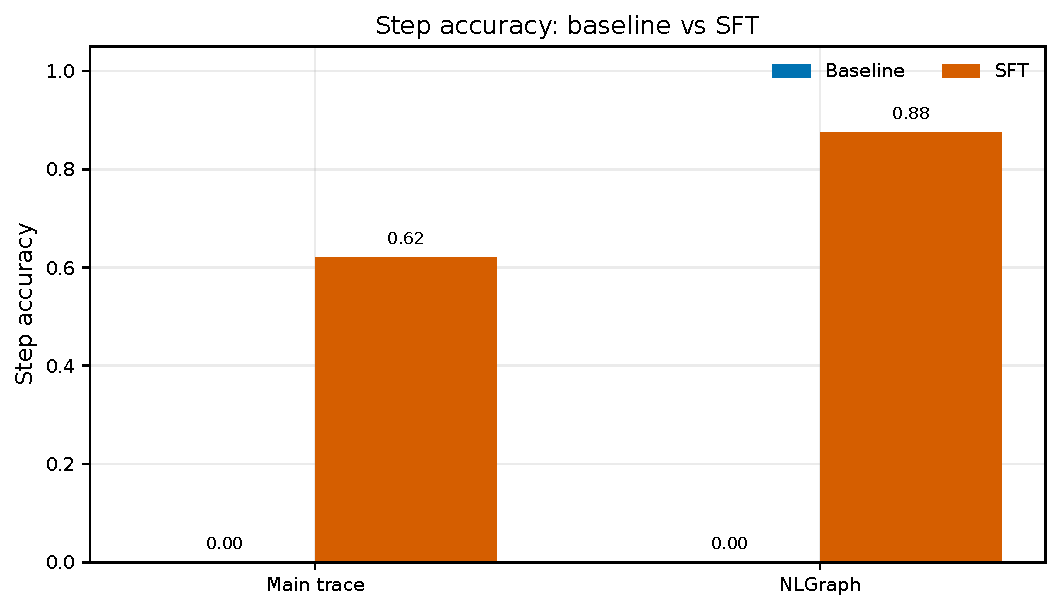
\includegraphics[width=\linewidth]{figures/fig_step_accuracy_overview.pdf}
  \caption{Baseline vs SFT step accuracy across main and benchmark adapters.}
  \label{fig:sft-overview}
\end{figure}

Beyond aggregate accuracy, first-error depth shifts from immediate failure in baseline to later failure under SFT.
This is visible in Figure~\ref{fig:first-error}, where error mass moves rightward (deeper in trace), indicating improved short-horizon control before drift occurs.

\begin{figure}[t]
  \centering
  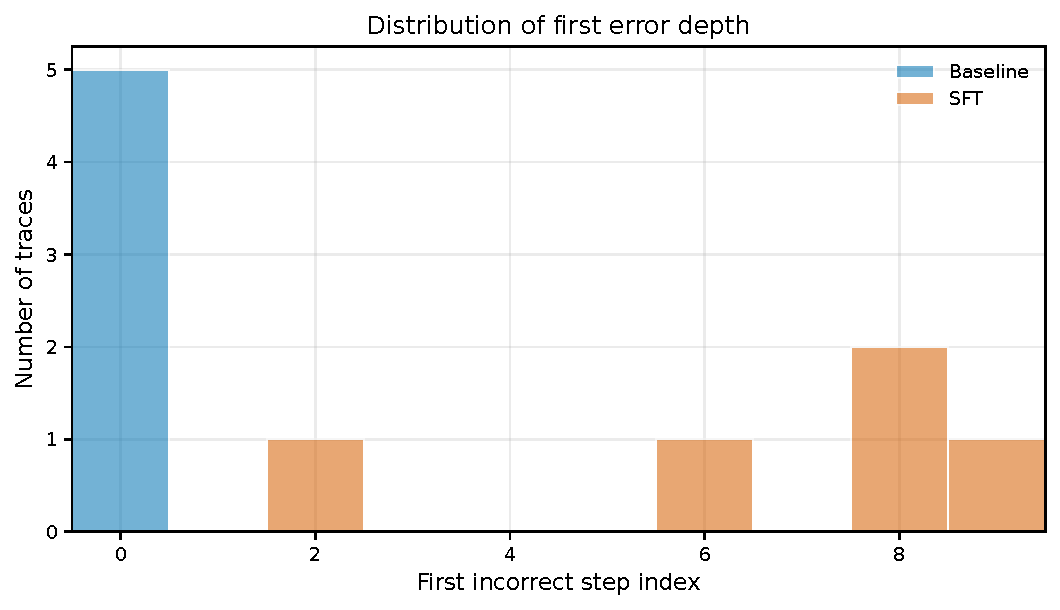
\includegraphics[width=\linewidth]{figures/fig_first_error_distribution.pdf}
  \caption{Distribution of first incorrect step, baseline vs SFT.}
  \label{fig:first-error}
\end{figure}

\subsection{Where failures occur}
Figures~\ref{fig:phase} and~\ref{fig:optype} characterize failure structure.
Phase analysis separates early/middle/late buckets; operation-type analysis highlights which gold operations are most error-prone.
Together they provide actionable supervision targets for stage-2 retraining.

\begin{figure}[t]
  \centering
  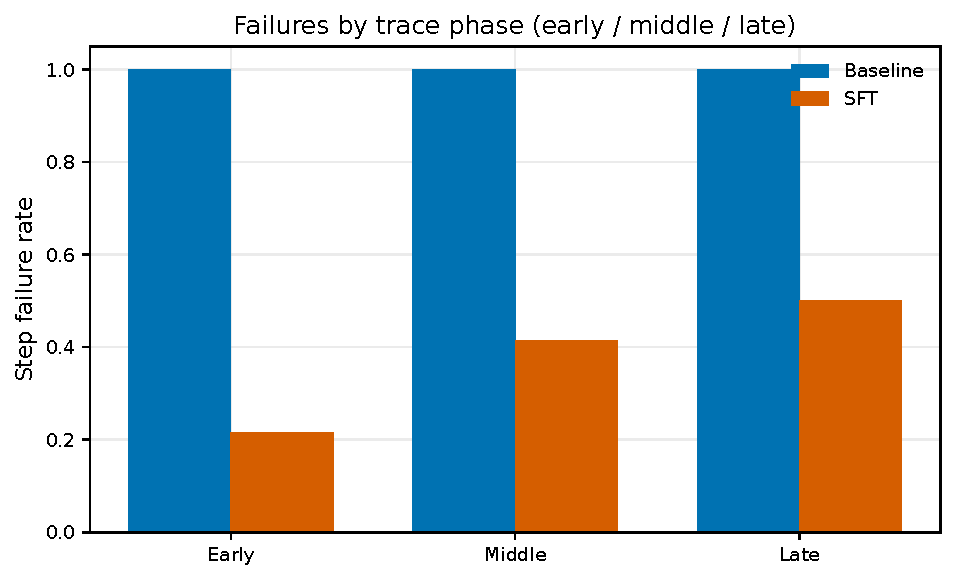
\includegraphics[width=\linewidth]{figures/fig_failure_by_phase.pdf}
  \caption{Failure rates by trace phase for baseline and SFT.}
  \label{fig:phase}
\end{figure}

\begin{figure}[t]
  \centering
  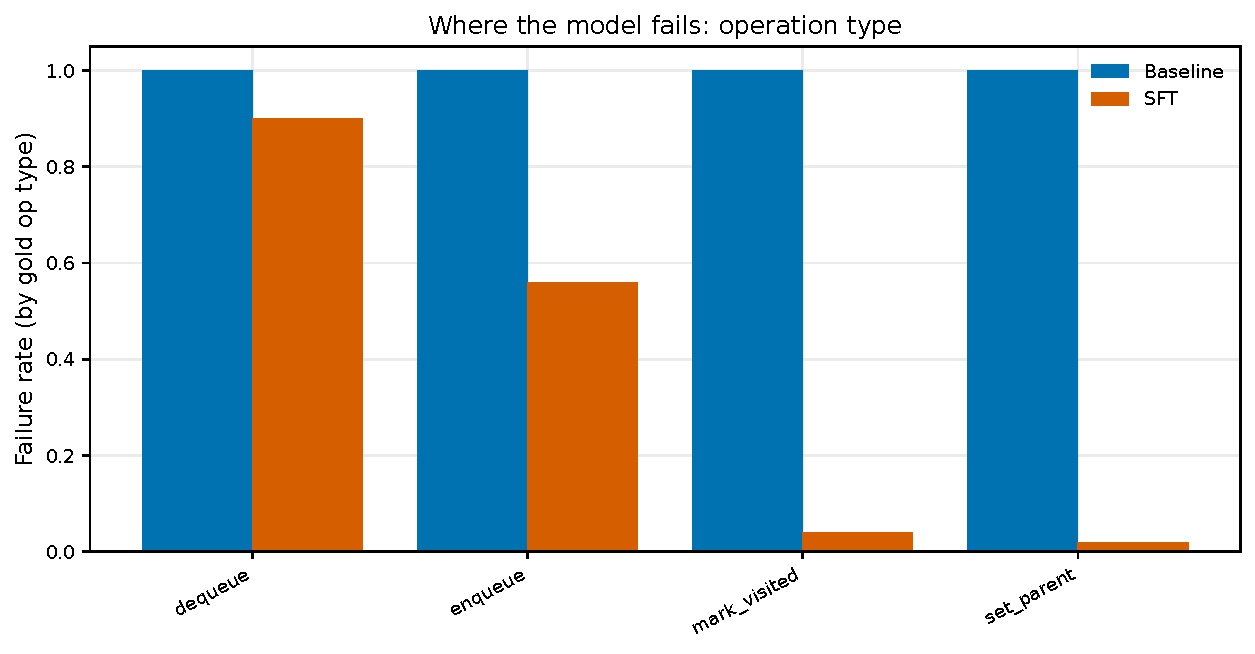
\includegraphics[width=\linewidth]{figures/fig_failure_by_operation_type.pdf}
  \caption{Failure rates by operation type (top categories).}
  \label{fig:optype}
\end{figure}

\subsection{Iterative pre/post retraining across algorithms}
Stage-2 retraining improves both BFS and DFS in the iterative runs.
For BFS, step accuracy increases 0.025 $\rightarrow$ 0.530 and failure rate drops 0.975 $\rightarrow$ 0.470.
For DFS, step accuracy increases 0.112 $\rightarrow$ 0.439 and failure rate drops 0.888 $\rightarrow$ 0.561.

These deltas are large in both absolute and relative terms.
BFS gains +0.505 absolute step accuracy (about 21$\times$ relative to pre accuracy), while DFS gains +0.327 absolute (about 3.9$\times$ relative).
Failure-rate decreases are similarly pronounced: roughly 52\% relative reduction for BFS and 37\% for DFS.
Given small sample counts, these should be interpreted as directional effect sizes rather than final population estimates, but they strongly justify continuation of error-driven retraining.

The central comparison appears in Figure~\ref{fig:cross-main}; delta-focused view appears in Figure~\ref{fig:cross-delta}.

\begin{figure}[t]
  \centering
  
\includegraphics[width=\linewidth]{figures/cross_algo/fig_cross_main_pre_post.pdf}
  \caption{BFS vs DFS core metrics before and after iterative retraining.}
  \label{fig:cross-main}
\end{figure}

\begin{figure}[t]
  \centering
  
\includegraphics[width=\linewidth]{figures/cross_algo/fig_cross_delta_bars.pdf}
  \caption{Post-minus-pre deltas for main and benchmark metrics.}
  \label{fig:cross-delta}
\end{figure}

NLGraph improves by +0.125 for both BFS and DFS in these runs.
GLBench remains flat at 0.000 pre/post, indicating either unresolved transfer mismatch, insufficient adaptation in current training scale, or dataset/adapter constraints requiring broader sweeps.

\subsection{Post-retraining failure dynamics}
Figure~\ref{fig:cross-phase-op} combines cross-algorithm phase and operation heatmaps.
The dominant trend is redistribution of error mass away from immediate failures while preserving non-trivial late-trace difficulty.
This is consistent with a model that learned better local recovery but has not yet eliminated long-horizon compounding behavior.

\begin{figure}[t]
  \centering
  \begin{subfigure}[t]{\linewidth}
    \centering
    
\includegraphics[width=\linewidth]{figures/cross_algo/fig_cross_failure_phase.pdf}
  \end{subfigure}
  \vspace{2mm}
  \begin{subfigure}[t]{\linewidth}
    \centering
    
\includegraphics[width=\linewidth]{figures/cross_algo/fig_cross_op_failure_heatmap.pdf}
  \end{subfigure}
  \caption{Failure-phase shifts and operation-type heatmap across BFS/DFS pre/post retraining.}
  \label{fig:cross-phase-op}
\end{figure}

Benchmark comparison and confusion concentration are summarized in Figures~\ref{fig:cross-bench} and~\ref{fig:cross-confusion}.
Confusion mass reduction post-retraining indicates fewer repeated high-frequency mistake patterns, even when absolute performance remains imperfect.

\subsection{Qualitative error trajectory interpretation}
The failure-analysis outputs align with observed pipeline behavior during development:
\begin{itemize}
  \item Baseline models frequently fail at or near step 0 with format-invalid or operation-invalid outputs.
  \item SFT shifts many errors later, indicating improved understanding of operation grammar and local policy.
  \item Stage-2 retraining most strongly reduces repeated confusion motifs that occur immediately after the first deviation.
\end{itemize}
This pattern supports the intuition behind the collection fix in \texttt{training/dagger.py}: invalid operations (\texttt{applied=False}) carry useful supervision signal and should not be discarded.
Once those examples were retained, stage-2 datasets became sufficiently populated to produce measurable post-retraining gains.

\begin{figure}[t]
  \centering
  
\includegraphics[width=\linewidth]{figures/cross_algo/fig_cross_benchmark_pre_post.pdf}
  \caption{NLGraph and GLBench pre/post behavior for BFS and DFS.}
  \label{fig:cross-bench}
\end{figure}

\begin{figure}[t]
  \centering
  
\includegraphics[width=\linewidth]{figures/cross_algo/fig_cross_confusion_mass.pdf}
  \caption{Concentration of top confusion counts before and after retraining.}
  \label{fig:cross-confusion}
\end{figure}

\begin{table*}[t]
  \centering
  \caption{Core metrics from committed run artifacts used in this report.}
  \label{tab:core}
  \begin{tabular}{lcccccc}
    \toprule
    Setting & Step Acc. & Failure Rate & Mean First Error & NLGraph & GLBench & Notes \\
    \midrule
    BFS baseline (base) & 0.000 & 1.000 & 0.0 & -- & -- & Main-task run in \texttt{out/} \\
    BFS SFT & 0.620 & 0.380 & 6.6 & 0.875* & 0.000 & Main + adapter eval in \texttt{out\_sft/} \\
    \midrule
    BFS pre-DAgger & 0.025 & 0.975 & 1.0 & 0.250 & 0.000 & Iterative summary (BFS run root) \\
    BFS post-DAgger & 0.530 & 0.470 & 1.0 & 0.375 & 0.000 & Iterative summary (BFS run root) \\
    BFS delta & +0.505 & -0.505 & 0.0 & +0.125 & 0.000 & Post minus pre \\
    \midrule
    DFS pre-DAgger & 0.112 & 0.888 & 1.0 & 0.250 & 0.000 & Iterative summary (DFS run root) \\
    DFS post-DAgger & 0.439 & 0.561 & 1.0 & 0.375 & 0.000 & Iterative summary (DFS run root) \\
    DFS delta & +0.327 & -0.327 & 0.0 & +0.125 & 0.000 & Post minus pre \\
    \bottomrule
  \end{tabular}
  \vspace{2pt}
  \footnotesize{*SFT NLGraph value comes from the committed adapter output with limited sample support; treat as directional.}
\end{table*}

\section{Alignment With Proposal and Development History}
The final system materially matches the proposal intent discussed through development:
\begin{itemize}
  \item \textbf{Decoupled logic/memory execution:} implemented with deterministic executor-in-the-loop inference.
  \item \textbf{Model adaptation:} SFT implemented and operational for core algorithms.
  \item \textbf{Failure-aware evaluation:} automated failure reports integrated into pipeline execution.
  \item \textbf{External benchmark hooks:} NLGraph and GLBench adapters integrated in the same pipeline.
  \item \textbf{Iterative recovery training:} DAgger-style collect/finetune/eval loop implemented with non-overwriting run management.
\end{itemize}

The development process also surfaced realistic systems challenges (environment compatibility, adapter format heterogeneity, pipeline fault tolerance), and the code now explicitly addresses these issues.
That robustness work is a meaningful deliverable for reproducible experimentation on shared HPC infrastructure.

\section{Reproducibility Checklist}
To support handoff and rerun reliability, this project now includes a practical reproducibility path:
\begin{itemize}
  \item \textbf{Single-entry evaluation script:} \texttt{scripts/run\_pipeline.sh} executes generation, inference, metrics, failure analysis, and optional benchmark adapters.
  \item \textbf{Iterative end-to-end driver:} \texttt{scripts/run\_iterative\_retraining\_pipeline.py} automates train/eval/collect/retrain/re-eval for one or more model configs.
  \item \textbf{Manifested outputs:} each pipeline run writes structured JSON metadata linking configuration and artifact paths.
  \item \textbf{Non-overwriting directory policy:} timestamped run roots plus \texttt{latest} symlink/copy handling preserve historical runs.
  \item \textbf{Paper-figure regeneration:} plotting scripts regenerate all figures from JSON artifacts into vector PDF for LaTeX.
\end{itemize}

For a final camera-ready study, we recommend freezing commit hash, config YAMLs, and exact command invocations in an appendix table; this can be generated directly from the produced run manifests.

\section{Threats to Validity}
\textbf{Small-sample reporting.}
Several cited artifacts use low sample counts for fast iteration.
Effects are large but confidence intervals are still wide.

\textbf{Benchmark incompleteness.}
GLBench remains near-zero in reported runs; this may reflect unresolved task mismatch or insufficient adaptation rather than intrinsic model incapability.

\textbf{Trace-length saturation.}
Despite gains, mean-first-error in iterative summaries remains shallow (around step 1 in pre/post aggregates), indicating persistent brittleness in fully free-running regimes.

\textbf{Model-family asymmetry.}
While both Qwen and Llama paths were engineered, not all comparisons currently run under a perfectly matched compute/data budget matrix.

\section{Future Work}
\subsection{Dijkstra as the next full experimental axis}
Dijkstra is the most important immediate extension because it introduces weighted, priority-sensitive transitions that stress both local operation selection and global consistency.
A complete Dijkstra campaign should include:
\begin{itemize}
  \item weighted-trace generation at larger scales and diverse degree distributions,
  \item operation-level taxonomies for \texttt{relax}, \texttt{settle}, and stale-frontier handling,
  \item iterative recovery training specialized to weighted shortest-path failure modes,
  \item structural generalization sweeps over graph size and weight distributions.
\end{itemize}

\subsection{Expanded training strategies}
The repository now also contains dedicated DPO/GRPO training entry points.
A natural next phase is to compare SFT-only vs SFT+preference optimization under the same executor-constrained interface, focusing on error localization and long-horizon robustness.

\subsection{Stronger statistical protocol}
Final publication-quality claims should use larger trace counts, multiple seeds, and explicit uncertainty reporting (bootstrap confidence intervals per metric), plus an ablation matrix over teacher-forced vs free-running settings.

\section{Conclusion}
This project delivers a full, working Graph of Thoughts experimentation stack rather than an isolated model checkpoint.
The system includes deterministic graph-state execution, SFT, failure-aware metrics, benchmark adapters, and automated iterative retraining.
Across committed artifacts, SFT and stage-2 recovery training produce substantial gains in BFS/DFS step accuracy and failure-rate reduction.

Equally important, the engineering outcomes --- robust pipeline orchestration, adapter-format handling, and reproducible figure generation --- make the project practical for continuation.
With expanded scale and full Dijkstra experiments, this framework is positioned to support stronger claims about LLM algorithmic reasoning under explicit state control.

\begin{thebibliography}{10}

\bibitem{got2024}
Maciej Besta et~al.
\newblock Graph of thoughts: Solving elaborate problems with large language models.
\newblock In \emph{Proceedings of the AAAI Conference on Artificial Intelligence}, 2024.

\bibitem{besta2024got}
Maciej Besta et~al.
\newblock Reasoning on graphs with large language models via graph-structured prompting.
\newblock \emph{arXiv preprint arXiv:2406.05673}, 2024.

\bibitem{wei2022cot}
Jason Wei et~al.
\newblock Chain-of-thought prompting elicits reasoning in large language models.
\newblock In \emph{Advances in Neural Information Processing Systems}, 2022.

\bibitem{liu2023lost}
Nelson F. Liu et~al.
\newblock Lost in the middle: How language models use long contexts.
\newblock \emph{Transactions of the Association for Computational Linguistics}, 2024.

\bibitem{hu2022lora}
Edward J. Hu et~al.
\newblock LoRA: Low-rank adaptation of large language models.
\newblock In \emph{International Conference on Learning Representations}, 2022.

\bibitem{schick2023toolformer}
Timo Schick et~al.
\newblock Toolformer: Language models can teach themselves to use tools.
\newblock In \emph{Advances in Neural Information Processing Systems}, 2024.

\bibitem{nlgraph2024}
Yiming Wang, Zhuosheng Zhang, and Rui Wang.
\newblock Can language models solve graph problems in natural language?
\newblock In \emph{Advances in Neural Information Processing Systems}, 2024.

\bibitem{glbench2024}
Zhikai Chen et~al.
\newblock GLBench: A comprehensive benchmark for graph with large language models.
\newblock \emph{arXiv preprint arXiv:2407.00869}, 2024.

\bibitem{ross2011dagger}
St\'ephane Ross, Geoffrey Gordon, and Drew Bagnell.
\newblock A reduction of imitation learning and structured prediction to no-regret online learning.
\newblock In \emph{Proceedings of AISTATS}, 2011.

\end{thebibliography}

\end{document}
